
\documentclass[11pt, oneside]{amsart}
\usepackage[font={sf}]{caption}
\usepackage[]{graphics}
\usepackage{graphicx}
\usepackage{epstopdf}
%\usepackage{hyperref}
%\hypersetup{breaklinks=true, colorlinks=true, citecolor=blue}
\usepackage{natbib}
\usepackage{color}
\usepackage{soul}
\usepackage{rotating}
\usepackage{tabularx}
\usepackage{longtable}
\usepackage{lscape}
\usepackage{array}
\usepackage{siunitx}
\sisetup{math-micro=\text{µ},text-micro=µ}
\usepackage{multirow}
\usepackage{setspace}
\usepackage{textcomp}
\usepackage{dcolumn}
\setlength{\LTcapwidth}{7in}
\usepackage{dcolumn}
\usepackage[margin=0.5in]{geometry}

 \bibpunct{(}{)}{,}{a}{}{,}
 \doublespacing
 \raggedright
 \setlength{\parindent}{15pt} 

\graphicspath{{./Figs/}}


\begin{document}
%\setcounter{secnumdepth}{0}


{ \Large \bf Supplementary Methods}

A novel analytical framework to quantify co-gradient and counter-gradient variation 

M.A. Albecker, G.C. Trussell, and K.E. Lotterhos

\hspace{3cm}

\tableofcontents
%\listoftables
\listoffigures

\newpage

\renewcommand\thesection{Supplemental Methods}

\section{1. Proof for $Cov_{GE}$}

The following equation is the standard approach to measure the covariance (Cov) between a pair of variables (here shown as x and y).

\begin{equation}
Sample\:Cov(x,y) =  \frac{\sum (x - \overline{x})(y - \overline{y})}{N-1}
\end{equation}

\begin{equation}
Population\:Cov(x,y) =  \frac{\sum (x - \si\micro_{x})(y - \si\micro_{y})}{N}
\end{equation}

In which N is the total number of samples, $\overline{x}$ is the sample mean of x, $\si\micro_{x}$ is the population mean of x, while $\overline{y}$ is the sample mean of y and $\si\micro_{y}$ is the population mean of y. 

The standard Cov(X,Y) equation cannot be directly applied to calculating $Cov(G,E)$, because in $Cov(G,E)$ we do not want to measure the covariance among every combination of genotypic and environmental effects, but only among the pairs of genotypic and environmental effects sourced from the same native environment. Therefore, we added the indicator variable ($I$) to ensure that only those data in which genotypes ($i$) are correctly matched to the environments ($j$) to which they were sourced (or are native to) are used to estimate Covariance.  $I_{ij} = 1$ when genotype is correctly matched with the environment to which it is native, and $I_{ij} = 0$ otherwise (See Fig. 1 in the main text). In keeping, we take the covariance between genotypic and environmental effects on phenotypes, across all genotype-environment pairs ($n_{gen}$ = $n_{env}$). This gives: 

\begin{equation}
Population\:Cov(G,E) =  \frac{1}{ \sum_{i=1}^{n_{gen}}  \sum_{j=1}^{n_{env}}(I_{ij})} (\sum_{i=1}^{n_{gen}}  \sum_{j=1}^{n_{env}}(\si\micro_{i} - \si\micro)(\si\micro_{j} - \si\micro)(I_{ij}))
\end{equation}


In this equation, $\si\micro_{i}$ is the population mean phenotype of the $i$th genotype, and $\si\micro_{j}$ is the population mean phenotype of the $j$th environment, and $\si\micro$ is the overall population mean phenotype.

To allow for comparisons across taxa, study systems, and environmental gradients, we sought to standardize $Cov(G,E)$. The typical approach to standardize covariance is correlation, which standardizes by the product of the standard deviation of the x and y variable ($\sigma_{x}$*$\sigma_{y}$). Here, we standardize by the variance in group means (instead of variance in all the data) because Cov(G,E) is based on covariance between the group means.
We use $\sigma_{\si\micro_{i}}$ to represent the population standard deviation in the group means for genotypic effects , and $\sigma_{\si\micro_{j}}$ to represent the standard deviation in the group means for the environmental effects.

However, the group means for environmental effects and the group means for genotypic effects are not independent of each other, because they are both calculated from the phenotypic means.

For example, the following standardization produces inaccurate results: 

\begin{equation}
Cor(G,E) = \frac{1}{ \sum_{i=1}^{n_{gen}}  \sum_{j=1}^{n_{env}}(I_{ij})} (\frac { \sum_{i=1}^{n_{gen}}  \sum_{j=1}^{n_{env}}(\si\micro_{i} - \si\micro)(\si\micro_{j} - \si\micro)(I_{ij})}{(\sigma_{\si\micro_{i}}*\sigma_{\si\micro_{j}})})
\end{equation}

Equation 4 produces inaccurate results in simulations (e.g., does not produce Cov(G,E) estimates between -1 and 1) because the standardization by $\sigma_{\si\micro_{i}}*\sigma_{\si\micro_{j}}$ assumes that G and E are independent, but in this case, they are not. Thus, we multiply this equation by a correction term $k$:

\begin{equation}
( \frac{1}{ \sum_{i=1}^{n_{gen}}  \sum_{i=1}^{n_{gen}}(I_{ij})} \frac {\sum_{j=1}^{n_{env}}(\si\micro_{i} - \si\micro)(\si\micro_{j} - \si\micro)(I_{ij})}{(\sigma_{\si\micro_{i}}*\sigma_{\si\micro_{j}})})*k
\end{equation}

When the correction factor $k$ is equal to the following, the result is constrained between -1 and 1:

\begin{equation}
k = max(\frac{\sigma_{\si\micro_{i}}}{\sigma_{\si\micro_{j}}},\frac{\sigma_{\si\micro_{j}}}{\sigma_{\si\micro_{i}}})
\end{equation}

For example, if $\sigma_{\si\micro_{i}} > \sigma_{\si\micro_{j}}$ and we apply $\frac{\sigma_{\si\micro_{j}}}{\sigma_{\si\micro_{i}}}$ to the above equation, the $\sigma_{\si\micro_{j}}$ terms cancel each other and the correction becomes: 

\begin{equation}
\sigma_{\si\micro_{i}} * \sigma_{\si\micro_{i}}= \sigma^2_{\si\micro_{i}}
\end{equation}


Which when applied to the correlation equation, can be written as: 
\begin{equation}
 \frac{1}{ \sum_{i=1}^{n_{gen}}  \sum_{i=1}^{n_{gen}}(I_{ij})} (\frac {\sum_{j=1}^{n_{env}}(\si\micro_{i} - \si\micro)(\si\micro_{j} - \si\micro)(I_{ij})}{\sigma^2_{\si\micro_{i}}})
\end{equation}

Thus, the Cov(G,E) is standardized by the variance in group means for genotypic effects or the variance in group means for environmental effects, whichever is greater. This standardization preserves the relationship between the genotypic and environmental effects in the data, while constraining Cov(G,E) to be between -1 and 1.
Thus, the population and estimated measures for standardized covariance (which we call $Cov_{GE}$) are as follows: 

\begin{equation}
Population\:  Cov_{GE} =   \frac{1}{ \sum_{i=1}^{n_{gen}}  \sum_{j=1}^{n_{env}}(I_{ij})}(\frac{\sum_{i=1}^{n_{gen}} \sum_{j=1}^{n_{env}}(\si\micro_{i} - \si\micro)(\si\micro_{j} - \si\micro)(I_{ij})}{max(\sigma^2_{\si\micro_{i}},\sigma^2_{\si\micro_{j}})})
\end{equation}

\begin{equation}
Sample\: \hat{Cov_{GE}} = \frac{1}{ \sum_{i=1}^{n_{gen}}  \sum_{j=1}^{n_{env}}(I_{ij})-1}(\frac{ (\sum_{i=1}^{n_{gen}}  \sum_{j=1}^{n_{env}}(\bar{y_{i}}-\bar{y})(\bar{y_{j}}-\bar{y})I_{ij}}{max( s^2_{\bar{y_{i}}}, s^2_{\bar{y_{j}}})})
\end{equation}

For the sample estimate, $\bar{y_{i}}$ is the estimated marginal mean phenotype for $i$th genotype, $\bar{y_{j}}$ is the estimated marginal mean phenotype for  $j$th  environment, and $\bar{y}$ is the estimated overall mean phenotype. $s^2_{\bar{y_{i}}}$  is the variance in the group mean phenotype for genotypic effects, while  $s^2_{\bar{y_{j}}}$ is the variance in the group mean phenotype for environmental effects.


\clearpage
\newpage

\section{2. Population Equations}

We used simulated data to measure sampling estimates of $\hat{Cov_{GE}}$ and $\bar\Delta_{GxE}$, which are shown in the main document. However, to validate these measures, we also calculated population parameters based on observed $Cov_{GE}$ when $\epsilon_{ijk}$ = 0 (Eqn. 4 in main text) and used the following equations to measure population parameters of $Cov_{GE}$ and $\bar\Delta_{GxE}$. See Supplemental Figure S2 below for simulation results showing agreement between sampling estimates and population parameter. 
 
\begin{equation}
Population\:  Cov_{GE} =   \frac{1}{ \sum_{i=1}^{n_{gen}}  \sum_{j=1}^{n_{env}}(I_{ij})}(\frac{\sum_{i=1}^{n_{gen}} \sum_{j=1}^{n_{env}}(\si\micro_{i} - \si\micro)(\si\micro_{j} - \si\micro)(I_{ij})}{max(\sigma^2_{\si\micro_{i}},\sigma^2_{\si\micro_{j}})})
\end{equation}

In this equation, $n_{gen}$ is the number of genotypes and $n_{env}$ is the number of environments. $\si\micro_{i}$ is the mean phenotype for genotype $i$, $\si\micro_{j}$ is the mean phenotype for environment $j$, and $ \si\micro$ is the overall mean phenotype. $I_{ij}$ is the indicator variable which equals one when genotype $i$ is correctly matched with the environment   $j$ to which it is native, and zero otherwise. Standard deviation of genotypic group means is indicated by $\sigma_{\si\micro_{i}}$ and standard deviation of environmental group means is $\sigma_{\si\micro_{j}}$. 

\begin{equation}
Population\:  \bar\Delta_{GxE} =   \frac{1}{ (n_{gen})(n_{env})}  \sum_{i=1}^{n_{gen}}\sum_{j=1}^{n_{env}}|\si\micro_{ij} - \si\micro_{i} - \si\micro_{j} + \si\micro|
\end{equation}

In this equation, $n_{gen}$ is the number of genotypes and $n_{env}$ is the number of environments. $\si\micro_{ij}$ is the mean phenotype for genotype $i$ in environment $j$, $\si\micro_{i}$ is the mean phenotype for each genotype, $\si\micro_{j}$ is the mean phenotype for each environment, and $\si\micro$ is the overall mean phenotype. There is no indicator variable, as all combinations of genotype and environment are used to calculate $ \bar\Delta_{GxE}$.

\clearpage
\newpage

\section{3. Imbalanced Designs}

For common garden experimental designs, there may be imbalance where there are unequal sample sizes or unequal numbers of genotypes for each native environment. Estimated marginal means reduce bias that may arise from unequal sample sizes within groups, thus do not affect $\hat{Cov_{GE}}$. However, because environment and genotype are treated as factors in the ANOVA to extract estimated marginal means, imbalanced numbers of genotypes (example shown in Supplemental Figure S7B below) introduce bias in the environmental means ($\bar{y_j}$ or $\si\micro$) and overall mean phenotype ($\bar{y}$ or $\si\micro$) (See B in the table below)  In fact, both studies analyzed in the main text have imbalanced numbers of genotypes. To correct for the bias, a second ANOVA model with native environment substituted for genotype can then be used to extract estimated marginal means to calculate unbiased ($\bar{y_{j}}$ or $\si\micro_{j}$) and($\bar{y}$ or $\si\micro$). The original model should be used to generate estimated marginal means for  ($\bar{y_{i}}$ or $\si\micro_{i}$). As shown in column C in the table below, this approach returns $\si\micro_{j}$ and $\si\micro$ to the values in balanced designs (A). 

\renewcommand\thefigure{T1}
\begin{table}[h]
\begin{center}
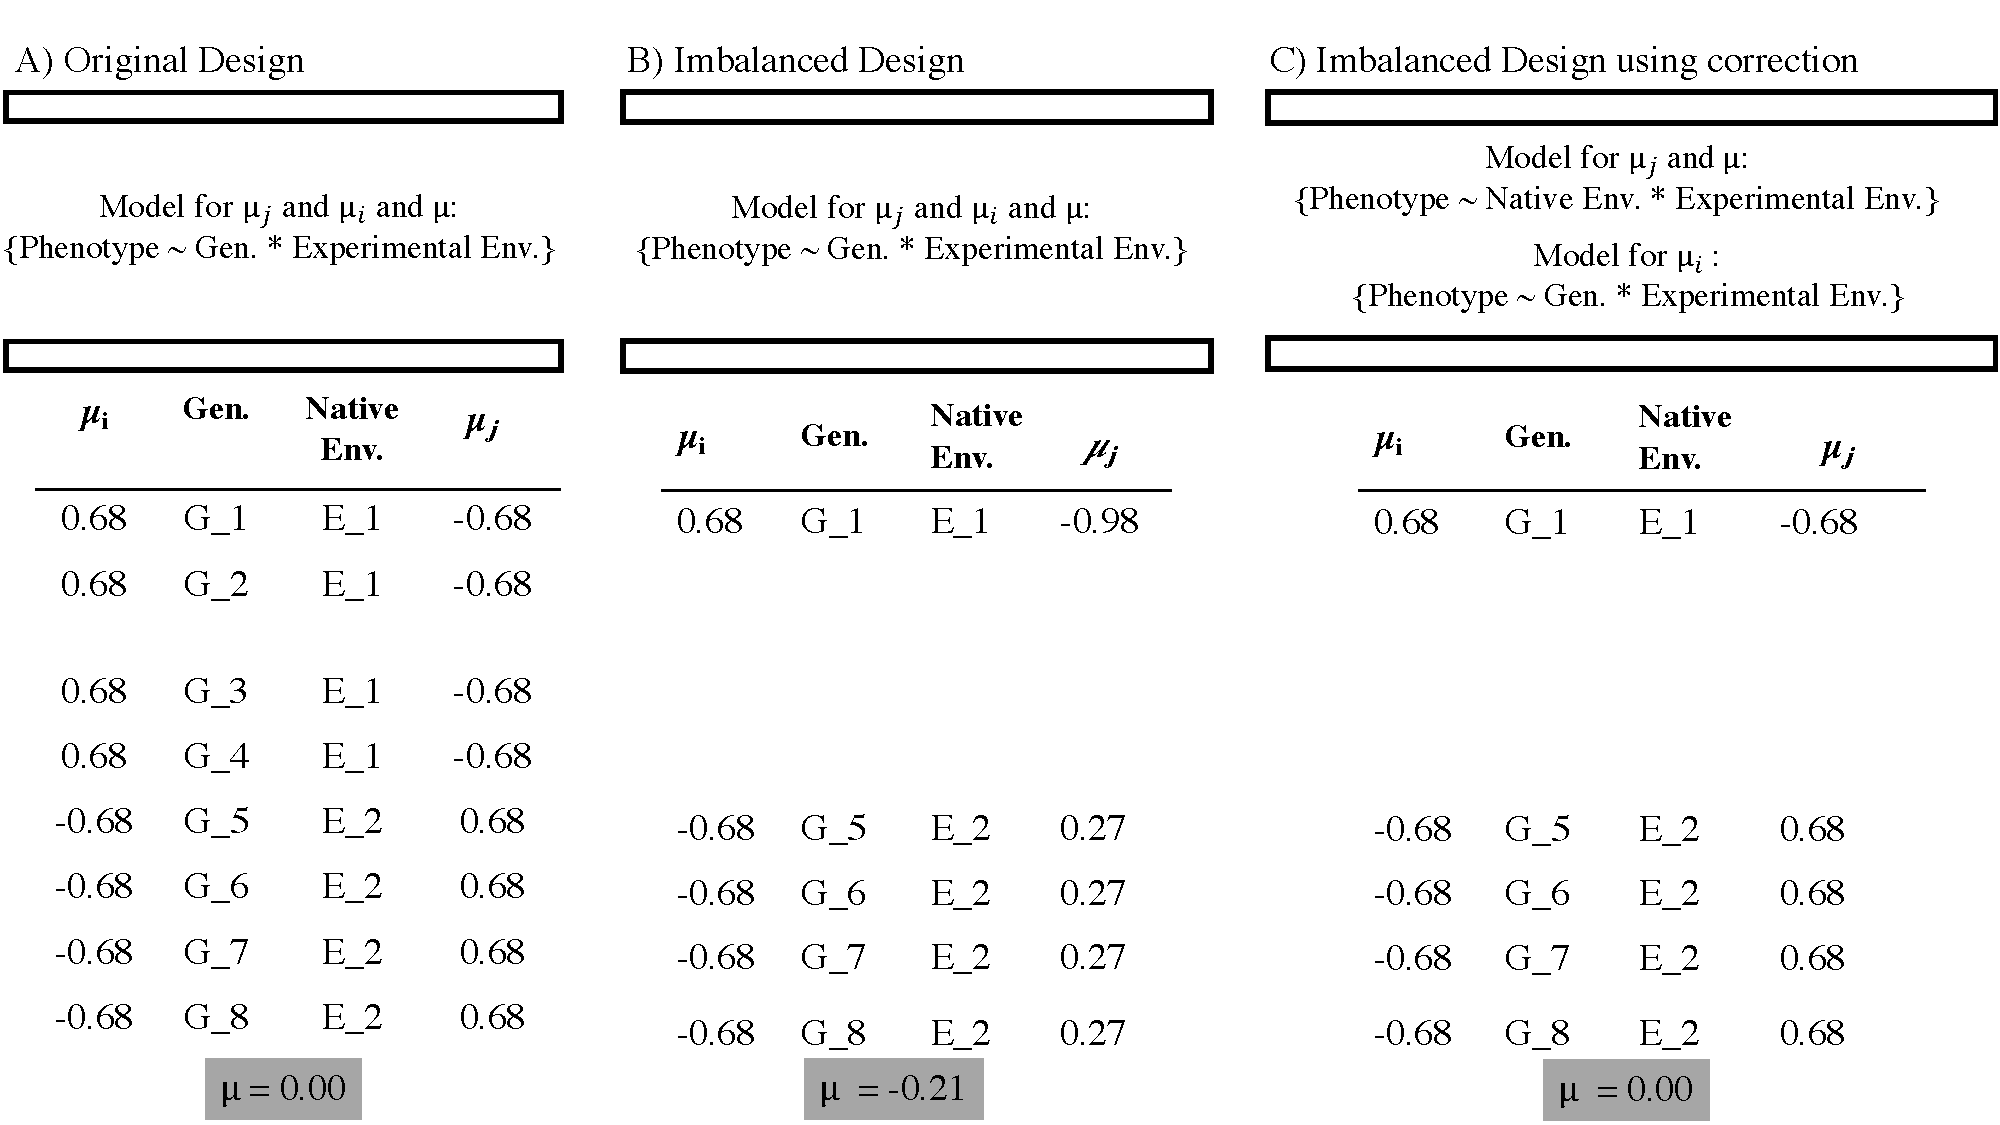
\includegraphics[width=6in]{Figs/UnbalancedTable.pdf}
\end{center}
\label{Table: Unbalanced Designs before and after correction}
\caption[Overall, genotypic, and environmental mean phenotypes]{(A) shows example data for a strong negative $Cov_{GE}$ pattern for a Common-garden design. When the design is balanced, four genotypes native to two different environments were measured across two experimental environments (Supplemental Figure S7 below for depiction of corresponding sample data, Fig. S7A shows data for panels A in the above table, Fig. S7B shows data for panels B and C in above table). When the design is balanced, the mean phenotypes for genotype ($\si\micro_{i}$), environment ($\si\micro_{j}$), and overall ($\si\micro$) are calculated by extracting estimated marginal means from a single model. When the design is unbalanced (as shown in B), continuing to use the same model to generate estimated marginal means produces bias in environmental means ($\si\micro_{j}$), and overall means ($\si\micro$). As shown in (C), the bias is corrected by conducting a secondary ANOVA with native environment replacing genotype to calculate environmental means ($\si\micro_{j}$), and overall means ($\si\micro$). Genotypic means ($\si\micro_{i}$) are calculated using the original ANOVA model.}
\end{table}
 
\clearpage
\newpage
\section{4. Variance partitioning}

In the main manuscript, we focus on estimating the effect size of $Cov_{GE}$ and $\bar\Delta_{GxE}$ and their significance. The effect size provides information about the strength of the pattern, which is a distinct type of information from the percent of variation in the phenotype explained by the following components: (i) genetic effects on phenotype, (ii) environmental effects on phenotypes, (iii) genetic x environment interactions, (iv) covariance between genetic and environmental effects on phenotypes, and (iv) residual error. Both Falconer (1989) and Conover and Schultz (1995) have previously discussed $Cov_{GE}$ in this more traditional sense as the percent of variation in the phenotype explained by different variance components:

\begin{equation}
V_P = V_G + V_E + V_{GxE} + xCov_{GE} 
\end{equation}

In a 2x2 reciprocal transplant or common garden design with 2 genotypes in 2 environments, $x = 2$. This factor of $x = 2$ does not extend to more complex designs, as explained below.

Here, we show how to extend sums of squares ($SS$) calculations from a traditional analysis of variance to incorporate $SS_{Cov_{GE}}$, which can in turn be used to understand the percent of variation in phenotypes explained by different components.  These calculations assume a fully factorial reciprocal transplant design. We do not advocate that these $SS$ be used to test the significance of the variance components with a traditional $F$-test, because the presence of $Cov_{GE}$ likely violates the assumption of independence among samples and complicates calculations of degrees of freedom (violations that are addressed in the main manuscript by using bootstrap and permutation for hypothesis testing). It is, however, useful to compare the percent of variation explained by different components to their effect sizes, because it furthers understanding of the relative influence of genetic differentiation and plasticity on the evolved patterns in the population.

In a reciprocal transplant experiment, there are $g$ genotypes transplanted into $e$ environmental patches, for a total of $g*e = n_{ge}$ genotype-environment combinations. In a fully factorial reciprocal transplant experiment, $g$ = $e$, $g$ is the number of levels of genotypes from $i = 1,2... g$, and $e$ is the number of levels of environments from $j = 1,2... e$.

Assuming the equal sample sizes $r$ (k = $1, 2, ...r$) within each genotype-environment combination, the following sums of squares can be estimated as:

\begin{equation}
V_G = SS_G = re\sum_{i=1}^g (\bar{y_i} - \bar{y})^2
\end{equation}

\begin{equation}
V_E = SS_E =  rg\sum_{j=1}^e (\bar{y_j} - \bar{y})^2 
\end{equation}

\begin{equation}
V_{GxE} = SS_{GE} = r \sum_{i=1}^g \sum_{j=1}^e (\bar{y_{ij}} - \bar{y_i} - \bar{y_j} + \bar{y})^2
\end{equation}

\begin{equation}
V_{Cov_{GE}}= SS_{Cov_{GE}} = | xr \sum_{i=1}^g\sum_{j=1}^e(\bar{y_i} - \bar{y})(\bar{y_j} - \bar{y})I_{ij} |
\end{equation}

\begin{equation}
V_{error} = SS_{Error} = \sum_{i=1}^g \sum_{j=1}^e \sum_{k=1}^r (y_{ijk}-\bar{y}_{ij})^2
\end{equation}
%it strikes me that the error is the same. shouldn't we be explaining some of it away with CovGE?

where $x = \frac{ge}{(\sum_{i=1}^g\sum_{j=1}^e I_{ij})}$, and $I_{ij}$ is an indicator variable that is 1 when the genotype $i$ originated from environment $j$ and 0 otherwise. In a 2x2 reciprocal transplant design, $g=2$, $e=2$, and $\sum_{i=1}^g\sum_{j=1}^e I_{ij}=2$, so $x = 2$ as is assumed in Eq. S1. However in a 4x4 reciprocal transplant design, $g=4$, $e=4$, and $\sum_{i=1}^g\sum_{j=1}^e I_{ij}=4$, so $x = 4$. The factor $x$ ensures that the $SS_{Cov_{GE}}$ scales appropriately with the $SS$ of the other components with the size of the experiment. Finally, since $Cov_{GE}$ can be negative under countergradient scenarios, we take the absolute value for partitioning variance.

The percent of variation explained by each component ($Comp$) can then be estimated as

\begin{equation}
\eta^2_{Comp} =  \frac{SS_{Comp}}{SS_G + SS_E + SS_{GxE} + SS_{CovGE} + SS_{Error}}
\end{equation}

We recognize that this is a crude approach. However, it provides a reasonable way to compare to the percent of variation explained by different components to their effect size estimates in the main text. For example, when $| Cov_{GE} |$ is maximized, equal amounts of non-residual variance are explained by $V_G$, $V_E$, and $V_{Cov_{GE}}$ for the fully factorial reciprocal transplant experiment with an arbitrary number of populations (Supplementary. Fig 6a). For this reason, when residual variation is minimized the maximum percent of phenotypic variance explained by $V_{Cov_{GE}}$ is rarely greater than 1/3 of the total phenotypic variance (Supplementary Fig. S5, Fig.S6a).

The comparison of effect sizes and variance components is also useful for understanding the relative influences of $V_G$ and $V_E$ on a particular value of $| Cov_{GE} |$; for instance, similarly intermediate values of $| Cov_{GE} |$ can be driven by higher $V_E$ and lower $V_G$ (Supplementary Fig. 6B), or lower $V_E$ and higher $V_G$ (Supplementary. Fig. S6c).


\clearpage
\newpage


\renewcommand\thesection{Supplemental Figures}


\section{Figures}

\renewcommand{\figurename}{Supplementary Figure}

\renewcommand\thefigure{S1}
\begin{figure}[h]
\begin{center}
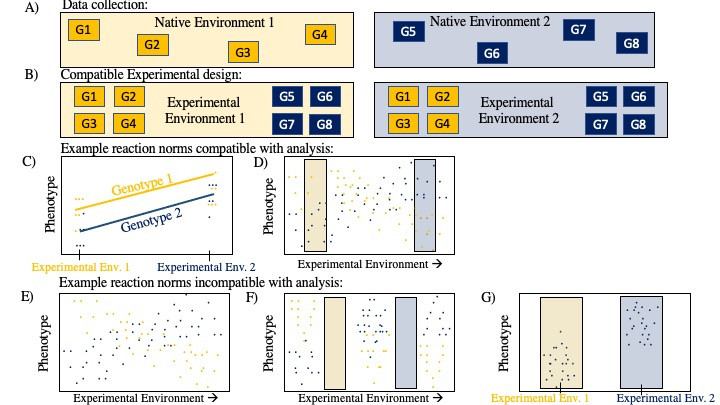
\includegraphics[width=6in]{Figs/IncompatibleDesigns.jpg}
\end{center}
\label{Fig: Compatible and Incompatible designs}
\caption[Examples of experimental designs that are compatible or incompatible with $Cov_{GE}$.]{Examples of experimental designs that are compatible or incompatible with $Cov_{GE}$. Plot A shows how phenotypic data are collected. Each box represents a different environment (orange, blue). Four genotypes are shown within each environment, with boxes representing the genotypes from which individuals (samples) are collected. Plot B shows an example of a fully factorial experimental design in which genotypes native to each environment are exposed to both environmental conditions. Plots C and D indicate phenotypic data that may result from the experimental design in panel B that are compatible with the analysis presented herein. Plot C shows categorical phenotypic data collected in either Environment 1 (orange), or Environment 2 (blue). Plot D shows phenotypic collected from an experimental design that used a continuous environmental gradient. However, to be analyzed, continuous phenotypic data would need to be binned. Note that in panel D, there are uneven numbers of samples in each bin. This is okay, because estimated marginal means reduce bias from unequal sample sizes. Plots E, F, and G show designs that are not incompatible with the $Cov_{GE}$ equation. Panel E shows phenotypic data along a continuous axis but there is no information on which environment each genotype is native to. Because our analysis requires that information on the native environment of each genotype is known, this design would remain incompatible even if environment was categorical (like in plot C). Plot F demonstrates phenotypic data in which the native environment is known, but was not included as a treatment in the experiment. Indeed, not only is information about the native environment required, but it also must be included as a treatment. Plot G shows an instance where a single genotype is tested across multiple environments. This design is incompatible because the $Cov_{GE}$ calculation requires at least 2 genotypes from at least 2 environments (but note that 2x2 designs are often underpowered - see Fig. 4 in the main text). }
\end{figure}

\clearpage
\newpage

\renewcommand\thefigure{S2}
\begin{figure}[h]
\begin{center}
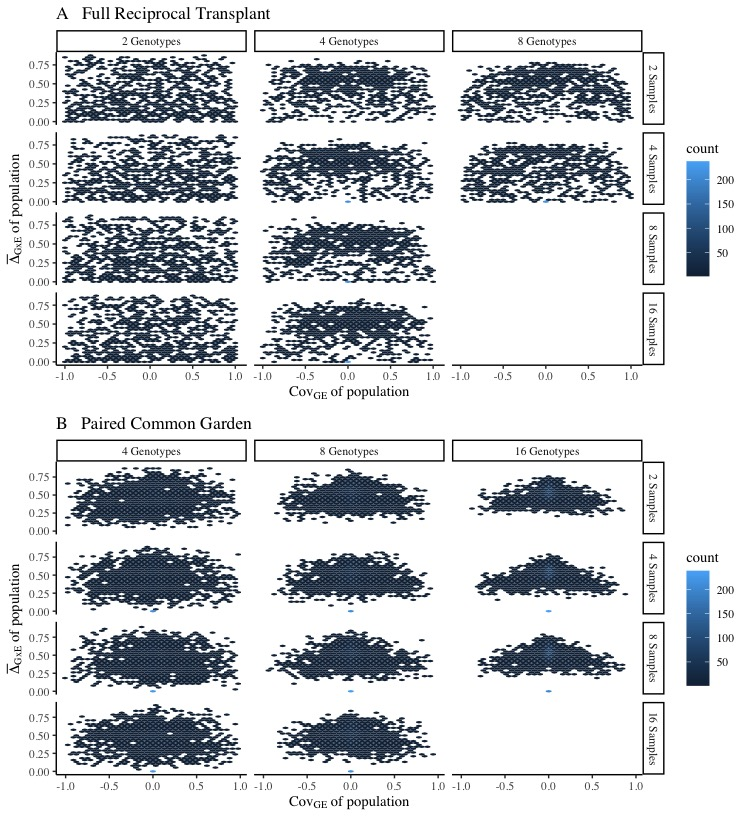
\includegraphics[width=6in]{Figs/HexPlot.jpeg}
\end{center}
\label{Fig: Parameter Coverage}
\caption[Coverage of parameter space of $Cov_{GE}$ and $\bar\Delta_{GxE}$ for full reciprocal transplant (A) and paired common garden designs (B).]{Coverage of parameter space of $Cov_{GE}$ and $\bar\Delta_{GxE}$ for full reciprocal transplant (A) and paired common garden designs (B). Hexagons are colored according to the density of observations in each bin. }
\end{figure}

\clearpage
\newpage


\renewcommand\thefigure{S3}
\begin{figure}[h]
\begin{center}
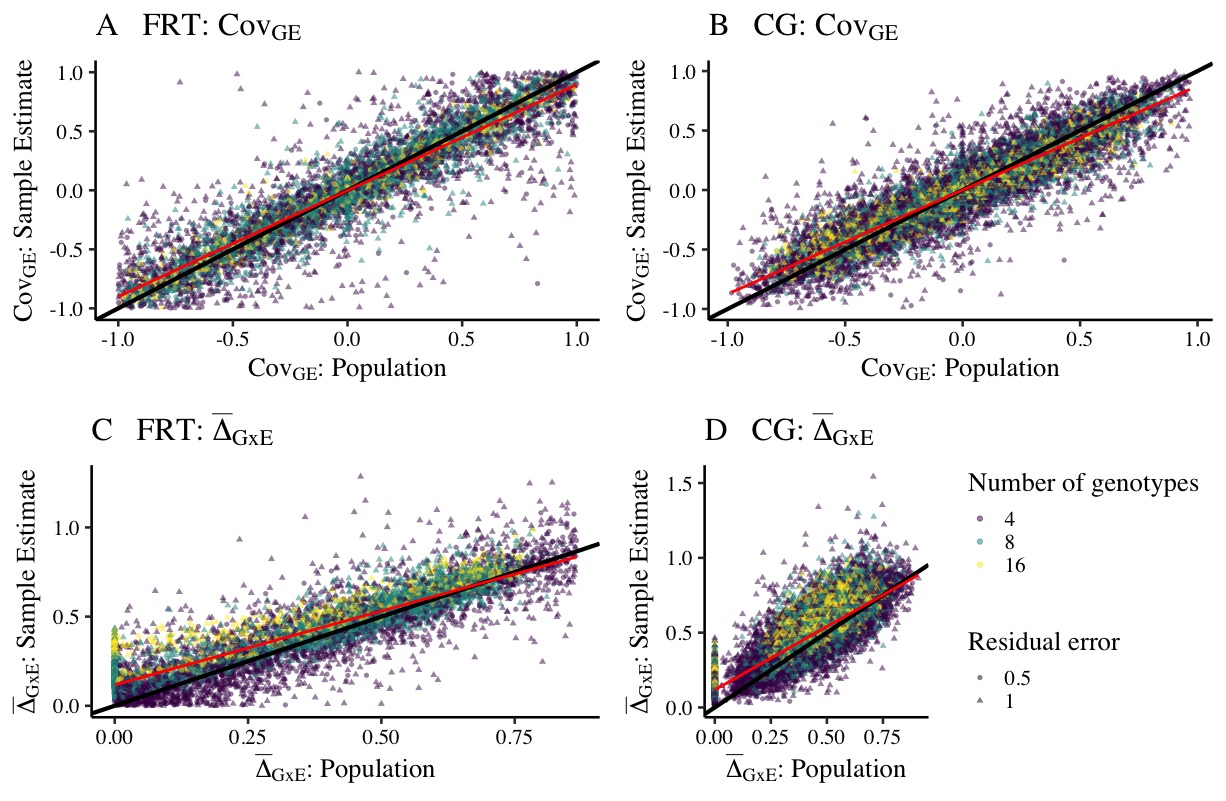
\includegraphics[width=6in]{Figs/SampleVsPopulation.jpeg}
\end{center}
\label{Fig: Population vs. Sample Estimates}
\caption[Agreement between population measures and sample estimates of  $\hat{Cov_{GE}}$ and $\bar\Delta_{GxE}$ for Full Reciprocal Transplant (A, C) and paired Common Garden designs (B, D). ]{Agreement between population measures and sample estimates of  $\hat{Cov_{GE}}$ and $\bar\Delta_{GxE}$ for Full Reciprocal Transplant (A, C) and paired Common Garden designs (B, D). The black line falls along a 1:1 line while the red line reflects the pattern of the data. Point colors indicate the number of genotypes, while point shapes indicate the level of residual variation. As expected, sample estimates deviate more from the population measure in situations with low sample sizes and higher residual variation.}
\end{figure}


\clearpage
\newpage
\renewcommand\thefigure{S4}
\begin{figure}[h]
\begin{center}
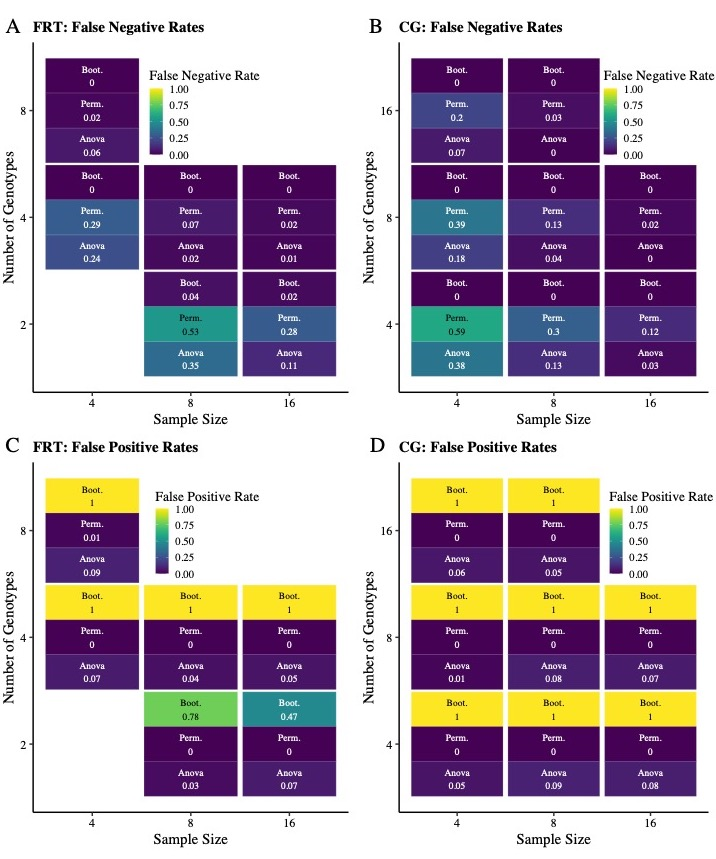
\includegraphics[width=6in]{Figs/GxE_Panel.jpg}
\end{center}
\label{Fig: }
\caption[False negative rates for $\bar\Delta_{GxE}$ for Full Reciprocal Transplant (A) and paired Common Garden designs (B) and false positive rates for full reciprocal transplant (C) and paired Common Garden designs (D). ] {Heat map showing false negative rates for $\bar\Delta_{GxE}$ for Full Reciprocal Transplant (A) and paired Common Garden designs (B) and false positive rates for full reciprocal transplant (C) and paired Common Garden designs (D). Tiles are split to show rates for bootstrapping (top), permutation (middle) and ANOVA (bottom) approaches. This figure complements Fig. 4 in the main text and is meant to demonstrate that bootstrapping produces unreliable confidence intervals for  $\bar\Delta_{GxE}$. }

\end{figure}

\clearpage
\newpage


\renewcommand\thefigure{S5}
\begin{figure}[h]
\begin{center}
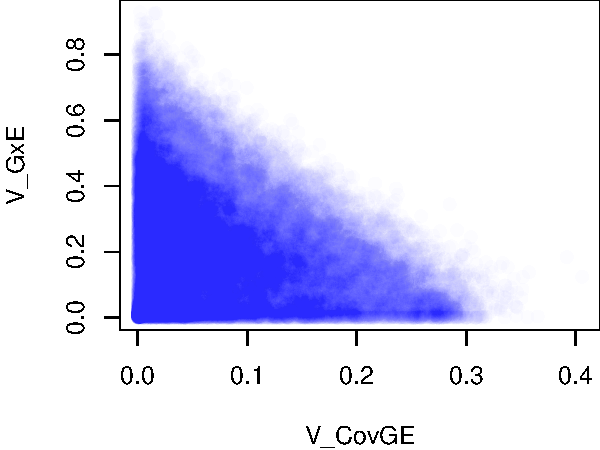
\includegraphics[width=6in]{Figs/VgxevsVcov.pdf}
\end{center}
\label{Fig: }
\caption[Comparison of the percent of variance explained by $V_{GxE}$ and $V_{Cov_{GE}}$ across all simulations.]{Comparison of the percent of variance explained by $V_{GxE}$ and $V_{Cov_{GE}}$ across all simulations.  }
\end{figure}

\clearpage
\newpage


\renewcommand\thefigure{S6}
\begin{figure}[h]
\begin{center}
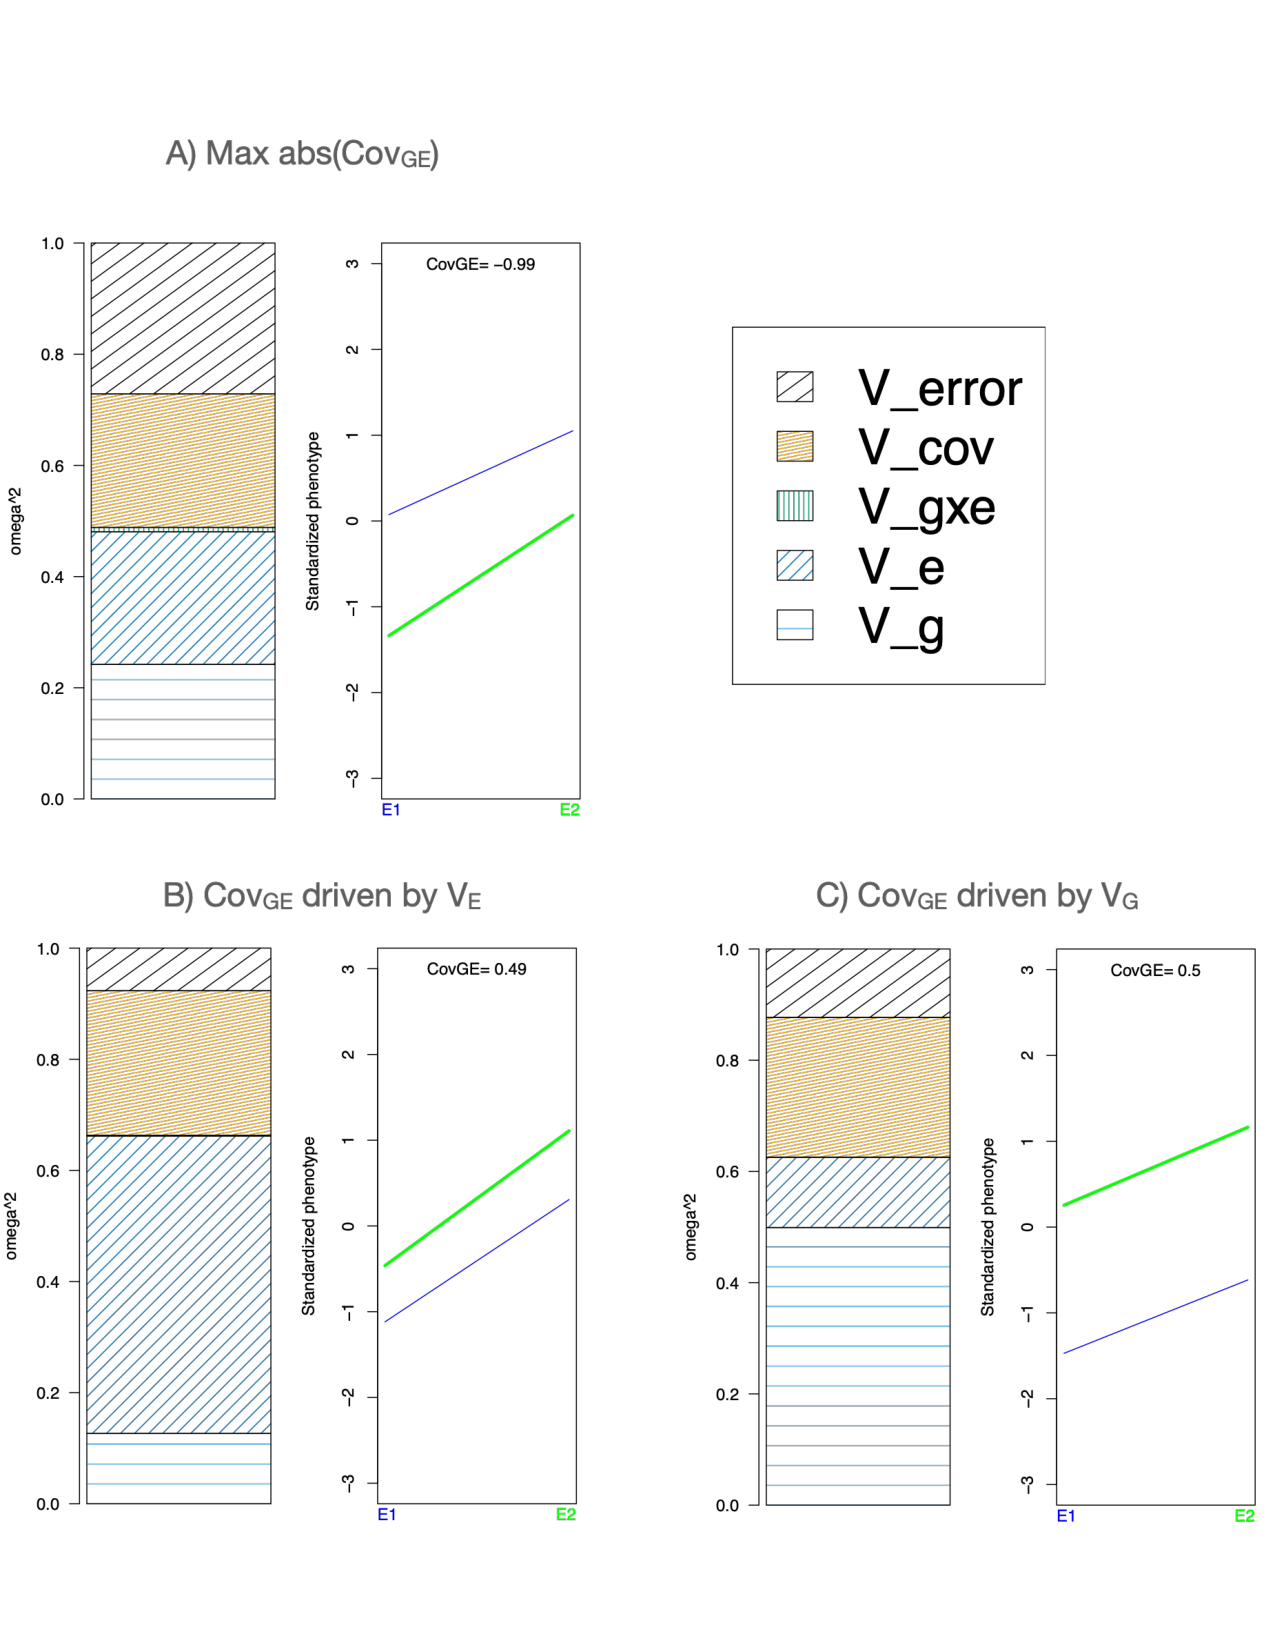
\includegraphics[width=6in]{Figs/EstimateVsVariance.pdf}
\end{center}
\label{Fig: }
\caption[Comparison of the percent of variance explained by $V_{Cov_{GE}}$ with the effect size $Cov_{GE}$ for three example simulations from a 2 genotype x 2 environment reciprocal transplant design.]{Comparison of the percent of variance explained by $V_{Cov_{GE}}$ with the effect size of $Cov_{GE}$ for three example simulations from a 2 genotype x 2 environment reciprocal transplant design. In each subpanel, the stacked barplot on the left of each panel shows the proportion of variance explained by each component corresponding to the legend (See Supplemental Materials 4), while the plot on the right shows the mean standardized reaction norms for each genotype (the effect size of $Cov_{GE}$ is shown at the top). A) When $| Cov_{GE} | = 1$ (i.e., maximal $Cov_{GE}$), equal proportions of phenotypic variance is explained by $V_G$, $V_E$, and $V_{Cov_{GE}}$. B) An intermediate effect size of  $Cov_{GE} = 0.5$ arising from larger $V_E$ compared to $V_G$.  C) An intermediate effect size of  $Cov_{GE} = 0.5$ arising from larger $V_G$ compared to $V_E$.  }
\end{figure}


\clearpage
\newpage

\renewcommand\thefigure{S7}
\begin{figure}[h]
\begin{center}
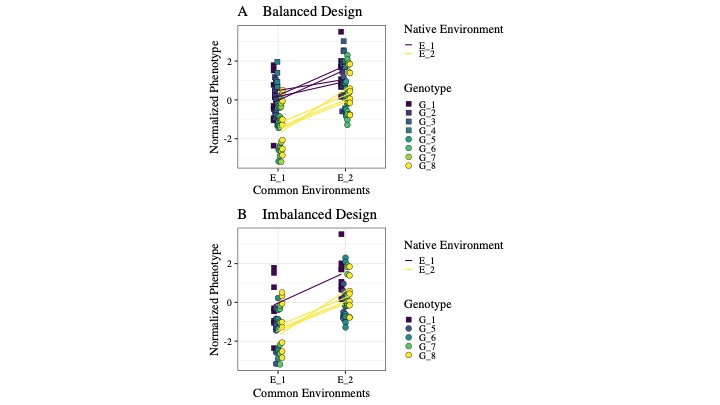
\includegraphics[width=6in]{Figs/Balanced_Imbalanced.jpg}
\end{center}
\label{Fig: }
\caption[Examples of sample data and reaction norms for balanced (A) vs. unbalanced designs (B) that correspond to Supplementary Table 1 above. ] {(A) An example of normalized phenotypic data for a balanced common garden design, meaning that both native environments have equal numbers of genotypes (in this case, 4 genotypes each). Points show phenotypic data colored according to genotype, while reaction norms are colored according to the environment to which the different genotypes are native. Data point shapes correspond to the native environment as well.  (B) Normalized phenotypic for an imbalanced design in which there are 4 genotypes native to Environment 2, but only 1 genotype native to Environment 1. Imbalanced designs can generate bias in $Cov_{GE}$ unless corrected. See Supplemental Methods 3 for details on the correction. }

\end{figure}

\clearpage
\newpage


\end{document}